\documentclass[10pt,letterpaper]{article}
\usepackage{opex3}
\usepackage{color}
\usepackage{threeparttable}
\usepackage{siunitx,graphicx,overpic,epstopdf,amsmath,amssymb,bm}
\usepackage{cite}
\usepackage{subcaption} 

%%%%%%%%%%%%%%%%%%%%%%% begin %%%%%%%%%%%%%%%%%%%%%%%%%%%%%%
\begin{document}
\graphicspath{{figures/}}

\title{Resolution comparison between integral imaging based hologram synthesis methods using rectangular and hexagonal lens arrays}

\author{Ni Chen,$^{1}$ Jiwoon Yeom,$^{1}$ Jae-Hyun Jung,$^{1}$ Jae-Hyeung Park,$^{2}$ and Byoungho Lee$^{1,*}$}

\address{$^{1}$School of Electrical Engineering, Seoul National University, Gwanak-Gu Gwanakro 1, Seoul 151-744, Korea.}
\address{$^{2}$School of Electrical \& Computer Engineering, Chungbuk National University, 410 SungBong-Ro, Heungduk-Gu Cheongju-Si, Chungbuk, 361-763, Korea.}

\email{$^*$byoungho@snu.ac.kr} %% email address is required


% \homepage{http:...} %% author's URL, if desired

%%%%%%%%%%%%%%%%%%% abstract and OCIS codes %%%%%%%%%%%%%%%%
%% [use \begin{abstract*}...\end{abstract*} if exempt from copyright]

\begin{abstract}
We compare the resolution of the hologram reconstruction synthesis methods based on integral imaging using rectangular and hexagonal lens arrays. By using a hexagonal lens array instead of conventional rectangular lens array, the three-dimensional objects are sampled with hexagonal grids. Due to more efficient sampling of the hexagonal grid, the resolution of the reconstructed object is higher compared with the case of using rectangular lens array. We analyze the resolution enhancement of the hologram reconstruction quantitatively and verify it experimentally.
\end{abstract}

\ocis{(090.0090) Holography; (100.6890) Three-dimensional image processing; (350.5730) Resolution.} % REPLACE WITH CORRECT OCIS CODES FOR YOUR ARTICLE, MINIMUM OF TWO; Avoid using the OCIS codes for “General” or “General science” whenever possible.
%For a complete list of OCIS codes, visit: http://www.opticsinfobase.org/submit/ocis/

%%%%%%%%%%%%%%%%%%%%%%% References %%%%%%%%%%%%%%%%%%%%%%%%%
\bibliographystyle{osajnl}
\bibliography{shref}

%%%%%%%%%%%%%%%%%%%%%%%%%%  body  %%%%%%%%%%%%%%%%%%%%%%%%%%
\section{Introduction}
Holography is an attractive autostereoscopic three-dimensional~(3D) display technique. It is able to provide flawless 3D images with complete human depth cues. However, the requirement of coherent system limits its application. Recently, digital hologram synthesis of 3D objects under incoherent illumination has been developed~\cite{Shaked_2009_AO,Park_2009_OE} although the basic concept of incoherent illumination is quite old~\cite{Pole_1967_APL}. A digital camera is used to capture multiple perspective images of 3D objects under incoherent illumination; the captured images are then digitally processed to synthesize the hologram. In these methods, integral imaging based method has its advantages in the points that all 3D information is captured with a single shot and the position of the reconstruction can be manipulated after capturing~\cite{Park_2009_OE}. However, the resolution of the reconstructed images is limited because it fundamentally relies on the sampling of the lens array. There are many researches for enhancing the resolution of reconstructed images in integral imaging or holograms generated based on integral imaging, such as time multiplexing method~\cite{Hong_2011_AO,Hong_2004_OL,Kishk_2003_OE}, synchronously moving micro-optics method~\cite{Hong_2004_OL,Jang_2002_OL}, micro lens array scanning method~\cite{Erdmann_2001_AO}, and lens array shift method~\cite{Chen_2010_OE,Lim_2009_OE}. These non-stationary lens array methods have demonstrated efficient resolution enhancement of integral imaging~\cite{Lee_2001_OL,Park_2009_AO}. However, they induced mechanical motion problem.

All these methods are based on the enhanced sampling of spatial-angular light ray distribution using non-stationary lens array. For the lens array, most of those methods use rectangular lens array and hence the light ray distribution is captured in a rectangular grid. However, hexagonal grid provides higher packing density and gives a more accurate approximation of circular regions compared with the rectangular grid. In addition, the sampling points of the hexagonal grid are uniformly connected in the sense that each sampling point is located at a fixed distance to all the six adjacent pixels. Hence, hexagonal grids have been used in a wide variety of research fields~\cite{Middleton_2005,Jurasinski_2006}. It has been known that circularly band limited signals are sampled more efficiently by hexagonal grids than by rectangular grids~\cite{Petersen_1962_IC,Murphy_1982_JOSA,Baronti_2001_SPIE}. It has also been reported to enhance the display resolution using the hexagonal sampling strategy~\cite{Park_2010_SPIE,Chen_2010_SPIE}. 

In this paper, we compare the resolution of the hologram reconstruction based on integral imaging with a rectangular lens array and a hexagonal lens array. A hexagonal lens array and a rectangular lens array are used in the elemental image capturing process, and holograms are generated from the captured information following the method presented in Ref.~\cite{Park_2009_OE}. Using hexagonal lens array corresponds to the hexagonal sampling of the 3D object and thus can accommodate more in bandwidth. Although there have been usages of hexagonal lens array in integral imaging, there has been no study on its usage for hologram generation based on integral imaging. Also, although Mishina et. al~\cite{Mishina_2006_AO} reported an analysis on the aliasing in the hologram generated using integral imaging, their hologram generation method is different from the method considered in this paper and hence their analysis cannot be applied in our work. To the authors' best knowledge, this is the first report that provides the quantitative analysis and experimental verification on the resolution enhancement of the hologram synthesis using hexagonal lens array. In Section 2, we analyze the resolution enhancement quantitatively. In Sections 3 and 4, simulation and experimental results are presented to verify the analysis.

\section{Fourier hologram generation using hexagonal lens array}

\subsection{Principle of Fourier hologram generation from orthographic images}
The principle of Fourier hologram generation based on integral imaging is depicted in Fig.~\ref{fig_1}. It includes two parts: one is the orthographic image generation process from the captured elemental images and the other is hologram generation process from the orthographic images. 

\begin{figure}[!htp]
\centering
\includegraphics[width=.8\columnwidth]{fig_1}
\caption{Principle of Fourier hologram generation using integral imaging. (a) Hologram generation process. (b) Parameter definition.}
\label{fig_1}
\end{figure}
Table 1 lists the parameter definitions in Fig.~\ref{fig_1}(b). In the first step, the elemental images of the objects are captured at the focal plane of a lens array. The captured elemental images are comprised of the perspective images of the 3D object, each of which is formed by the corresponding elemental lens of the lens array. The orthographic images $P_s,t$ are generated by collecting the pixels that have the same local position $\theta=\tan^{-1}(s/l)\approx s/l$, $\varphi=\tan^{-1}(t/l)\approx t/l$ in each elemental image. The second step is generating a Fourier hologram from the orthographic images. For each orthographic image $P_s,t$, the phase factor of a plane wave with the corresponding projection angle is multiplied. The product is integrated into one pixel in the Fourier hologram plane as shown in Fig.~\ref{fig_1}(a). By repeating this process to all orthographic images the Fourier hologram can be generated~\cite{Park_2009_OE}. This Fourier hologram $O(u,v)$ generation procedure can be represented by the following~\cite{Park_2009_OE}: 

\begin{align}
O(u,v)
&=O(Ms,Mt) \nonumber\\ 
&=\int\int P_{s,t}(x_p, y_p)\exp(-j2\pi b(x_p s+y_p t)) dx_p dy_p, 
\label{Eq_1} 
\end{align} 
where 
\begin{align}
M=-\frac{2f}{l}, b=\frac{2}{\lambda l} , 
\label{Eq_2} 
\end{align} 
and $M$ is the magnification factor. It has been shown that the complex function $O(u,v)$ synthesized by using Eq.~\eqref{Eq_1} is equivalent to the Fourier hologram of the captured object~\cite{Park_2009_OE}. The synthesized hologram $O(u,v)$ is discretized with $\Delta u =M\Delta s=2f\Delta\theta$ and $\Delta v= M \Delta t=2f\Delta\varphi$ and the size of the hologram is given by $2L_u=2Ms_{max}=4f\theta_{max}$ and $2L_v=4f\varphi_{max}$~\cite{Kishk_2003_OE}.

\begin{table}[ht!]
\centering\caption{Parameter definition}
% \begin{tabular}{|p{0.5in}|p{1.6in}|p{0.5in}|p{1.8in}|} 
\begin{tabular}{lp{1.7in}|lp{1.7in}} 
\hline 
Parameter                & Description         & Parameter      & Description \\ \hline 
$l$                      & Focal length of the lens array       & $\Delta\theta, \Delta\varphi$ & Projection angle interval of the pixels in the elemental images \\ \hline 
$\Delta x_p, \Delta y_p$ & Lens pitch of lens array & $\theta_{max}, \varphi_{max}$ & Maximum projection angle \\ \hline 
$\Delta s, \Delta t$     & Pixel pitch of the element images & $u, v$ & Coordinates of generated hologram \\ \hline 
$s, t$                     & Local position of pixels in each elemental image & $f$ & Focal length of Fourier transform lens \\ \hline 
\end{tabular}
\label{tb_param}
\end{table}

\subsection{Comparison of conventional rectangular lens array sampling and hexagonal lens array sampling}
\begin{figure}[htb]
% \centering\includegraphics[width=.4\columnwidth]{fig_2}
\centering
	\captionsetup[subfigure]{justification=centering}
	\begin{subfigure}[b]{0.3\linewidth}
	\centering
	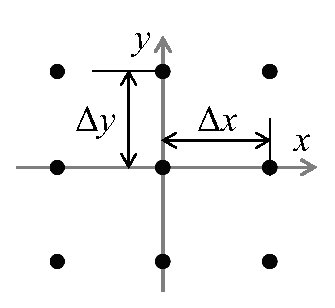
\includegraphics[width=1\columnwidth]{fig2_a}
	\caption{}
	\end{subfigure}
	\begin{subfigure}[b]{0.3\linewidth}
	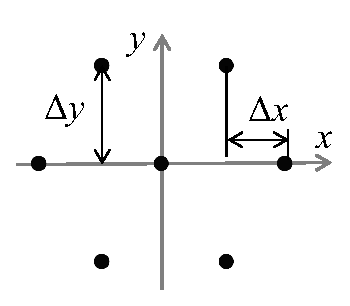
\includegraphics[width=1\columnwidth]{fig2_b}
	\centering
	\caption{}
	\end{subfigure}
\caption{Sampling in spatial domain. (a) Rectangular sampling grid. (b) Hexagonal sampling grid.}
\label{fig_2}
\end{figure}

Figure~\ref{fig_2} shows the rectangular sampling and hexagonal sampling. The sampling intervals $\Delta x$ and $\Delta y$ are defined as the distances between two adjacent columns and two adjacent rows, respectively. For an object field of $o(x, y)$, the rectangular sampled object field $\tilde{o}_{rec}(x, y)$ and hexagonal sampled object field $\tilde{o}_{hex}(x, y)$ can be described by Eqs.~\eqref{Eq_3} and \eqref{Eq_4}, respectively:
\begin{align}
\tilde{o}_{rec} (x,y)=\sum _{m,n}o(x,y)\delta (x-m\Delta x)\delta (y-n\Delta y) , 
\label{Eq_3} 
\end{align} 
\begin{align}
\tilde{o}_{hex} (x,y)=\sum _{m,n}o(x,y)\delta \left(x-(2m+n)\Delta x\right) \delta (y-n\Delta y). 
\label{Eq_4} 
\end{align}

In the Fourier hologram generation based on integral imaging, we define the lens pitch of the lens array as the distance between the centers of two adjacent lenses, as Fig.~\ref{fig_3} shows. Suppose a rectangular lens array and a hexagonal lens array have the same lens pitch $p$. Using these two lens arrays, integral Fourier holograms are generated with the method described in Section 2.1. Note that in the integral Fourier hologram method the orthographic image is generated by extracting single pixel per each elemental image. Hence the object field is first sampled with the lens array in the orthographic image generation step and this affects the final hologram resolution. 
\begin{figure}[htb]
% \centering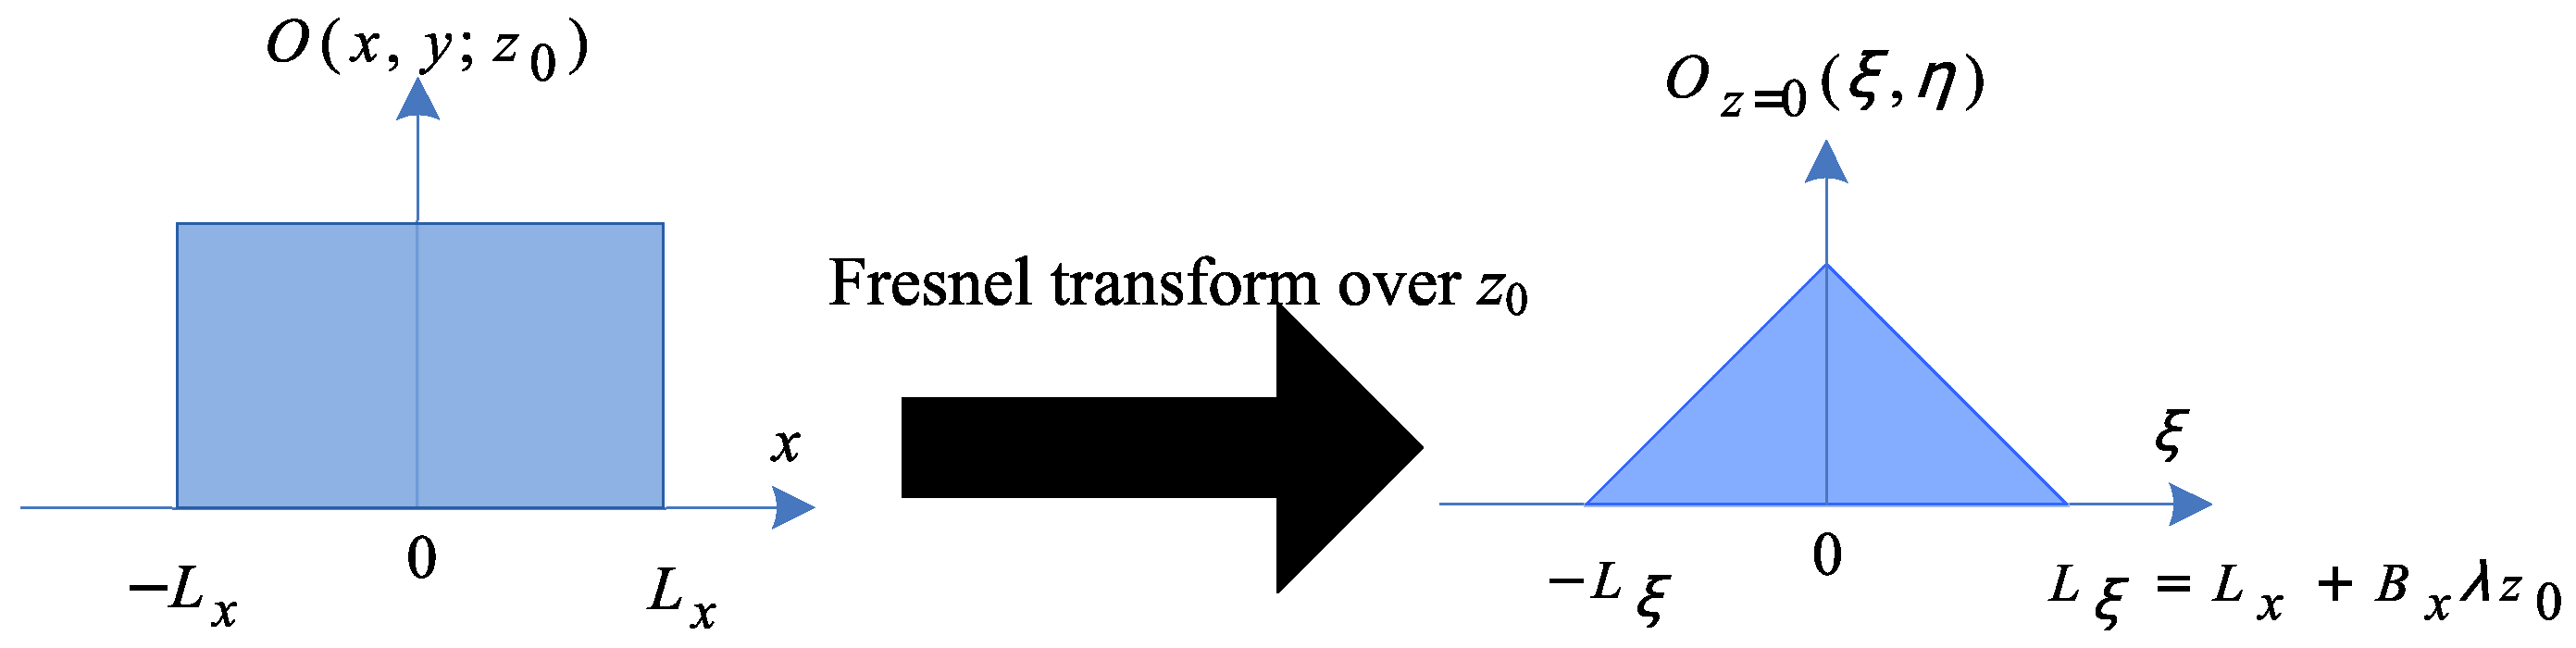
\includegraphics[width=.5\columnwidth]{fig_3}
\centering
	\captionsetup[subfigure]{justification=centering}
	\begin{subfigure}[b]{0.35\linewidth}
	\centering
	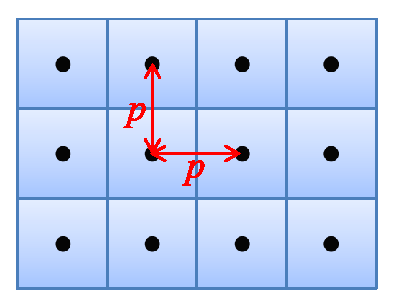
\includegraphics[width=1\columnwidth]{fig3_a}
	\caption{}
	\end{subfigure}
	\begin{subfigure}[b]{0.35\linewidth}
	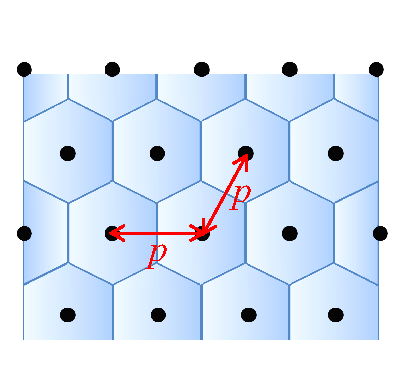
\includegraphics[width=1\columnwidth]{fig3_b}
	\centering
	\caption{}
	\end{subfigure}
\caption{Sampling with lens array. (a) Sampling by rectangular lens array. (b) Sampling by hexagonal lens array.}
\label{fig_3}
\end{figure}

The original object is sampled with rectangular or hexagonal lens array, as shown in Eqs.~\eqref{Eq_3} and \eqref{Eq_4}. The sampling interval is $\Delta x= \Delta y=p$ in the rectangular sampling and $\Delta x= p/2$ and $\Delta y=\sqrt{3}/2p$ in the hexagonal sampling. We analyzed the lateral size and the spatial frequency bandwidth of the reconstruction using these two types of lens arrays.  

Suppose the original object has a limited size $2L_x\times 2L_y$. As the reconstruction is the inverse Fourier transform of the hologram and the hologram is discretized with $\Delta u$ and $\Delta v$, by the sampling theory, the reconstruction is a repetition of the original object field. The repetition period is given by $\lambda f/\Delta u= \lambda f/M\Delta s= \lambda f/2f\Delta\theta = \lambda/(2\Delta\theta)$ along the horizontal direction and $\lambda f/\Delta v= \lambda f/M\Delta t= \lambda f/2f\Delta\varphi= \lambda/(2\Delta\varphi)$ along the vertical direction~\cite{Goodman_2005}, as Fig. 4 shows. In order to avoid overlapping in the reconstruction, the object size should be smaller than this repetition period. Thus the maximum size of the object that can be reconstructed without overlapping can be described as  
\begin{align}
2L_{x'} =\frac{\lambda}{2\Delta\theta} ,\, 2L_{y'} =\frac{\lambda}{2\Delta\varphi}. 
\label{Eq_5} 
\end{align} 

Because the projection angle intervals $\Delta\theta=\Delta s/l$ and $\Delta\varphi=\Delta t/l$ are only related to the pixel pitch of the capturing sensor, the maximum sizes of the reconstructed object are the same for the rectangular lens array case and hexagonal lens array case when the image sensors are the same.
\begin{figure}[htb]
\centering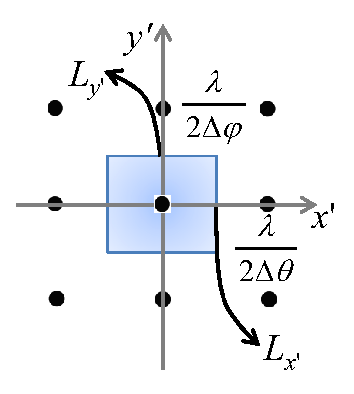
\includegraphics[width=.25\columnwidth]{fig_4}
\caption{Spatial domain representation of the reconstruction.}
\label{fig_4}
\end{figure}

The spatial frequency bandwidth of the reconstruction is determined by two factors; i.e., sampling of the object field with the lens array grid in the orthographic image generation step and the limited lateral size of the synthesized Fourier hologram. The sampling of the object field makes the reconstruction spectrum be replicas of the spatial frequency spectrum of the unsampled object field. The limited lateral size of the synthesized Fourier hologram defines cut-off spatial frequency in this spectrum.  

Let us first consider the effect of the sampling in the orthographic image generation. The spectrum of the sampled object field is given by
\begin{align} 
FT\left[\tilde{o}_{rec} \left(x,y\right)\right]=FT[o(x,y)]\otimes \sum _{m,n}\delta \left(f_x -\frac{m}{p} \right)\delta \left(f_{y} -\frac{n}{p} \right),  
\label{Eq_6}
\end{align} 
\begin{align} 
FT\left[\tilde{o}_{hex} \left(x,y\right)\right]=FT[o(x,y)]\otimes \sum _{m,n}\delta \left(f_x -\frac{2m+n}{p} \right)\delta \left(f_{y} -\frac{n}{\sqrt{3} p} \right), 
\label{Eq_7} 
\end{align} 
for rectangular lens array and hexagonal lens array, respectively and $\otimes$ represents convolution. Equations \eqref{Eq_6} and \eqref{Eq_7} show that the spectrum of the object field is repeated with different grid as depicted in Fig.~\ref{fig_5}. Therefore the maximum radial spatial frequency that can be reconstructed without aliasing is given by
\begin{align}  
f_{\rho,rec} =\sqrt{f_x^2 +f_y^2} \le \frac{1}{2p}, \nonumber \\ 
f_{\rho ,hex} =\sqrt{f_x^2 +f_y^2} \le \frac{1}{\sqrt{3} p} ,
\label{Eq_8}
\end{align} 
for rectangular lens array and hexagonal lens array case, respectively. The maximum spatial frequency is $f_{\rho,rec}=1/2p$ and $f_{\rho,hex}=1/\sqrt{3}p$. Hence, the resolution enhancement of a ratio $f_{\rho,hex}/f_{\rho,rec}=2/\sqrt{3}$ can be expected in hexagonal lens array case in comparison with the rectangular lens array case.

The limited lateral size of the Fourier hologram defines the cut-off spatial frequency of the reconstruction. The horizontal and vertical sizes $L_u$ and $2L_v$ of the synthesized Fourier hologram $O(u,v)$ are determined by the maximum projection angle in the orthographic image generation. From the geometry of the lens array, the synthesized Fourier hologram in the rectangular lens case has a rectangular shape of the lateral size $2L_u=4f\theta_{max}=2{fp}/l$ and $2L_v=4f\varphi_{max}=2{fp}/l$. On the contrary, it has a hexagonal shape of the lateral size $2L_u=4f\theta_{max}=2{fp}/l$ and $2L_v=4f\varphi_{max}=4{fp}/\sqrt{3l}$ in hexagonal lens case. The cut-off spatial frequency area is then given by the same shape as that of the generated hologram with their horizontal size $2f_x,_{max}=2L_u/\lambda f=2p/l\lambda$ and vertical size $2f_y,_{max}=2L_v/\lambda f=2p/l\lambda$ in rectangular lens array case and $2f_x,_{max}=2L_u/\lambda f=2p/l\lambda$ and vertical size $2f_y,_{max}=2L_v/\lambda f=4p/\sqrt{3}{l\lambda}$ in hexagonal lens array case as shown in green lines in Fig.~\ref{fig_5}. Then in the case of no aliasing~(due to sufficiently small elemental lens pitch p), the maximum spatial frequency range that can be reconstructed is slightly larger in the case of rectangular lens array. However, in case of aliasing as shown in Fig.~\ref{fig_5}, the hexagonal shape spatial frequency range reduces the amount of the aliasing with the same elemental lens pitch p  and the object bandwidth, presenting better image quality than the rectangular lens array. 
% \begin{figure}[htb]
% \centering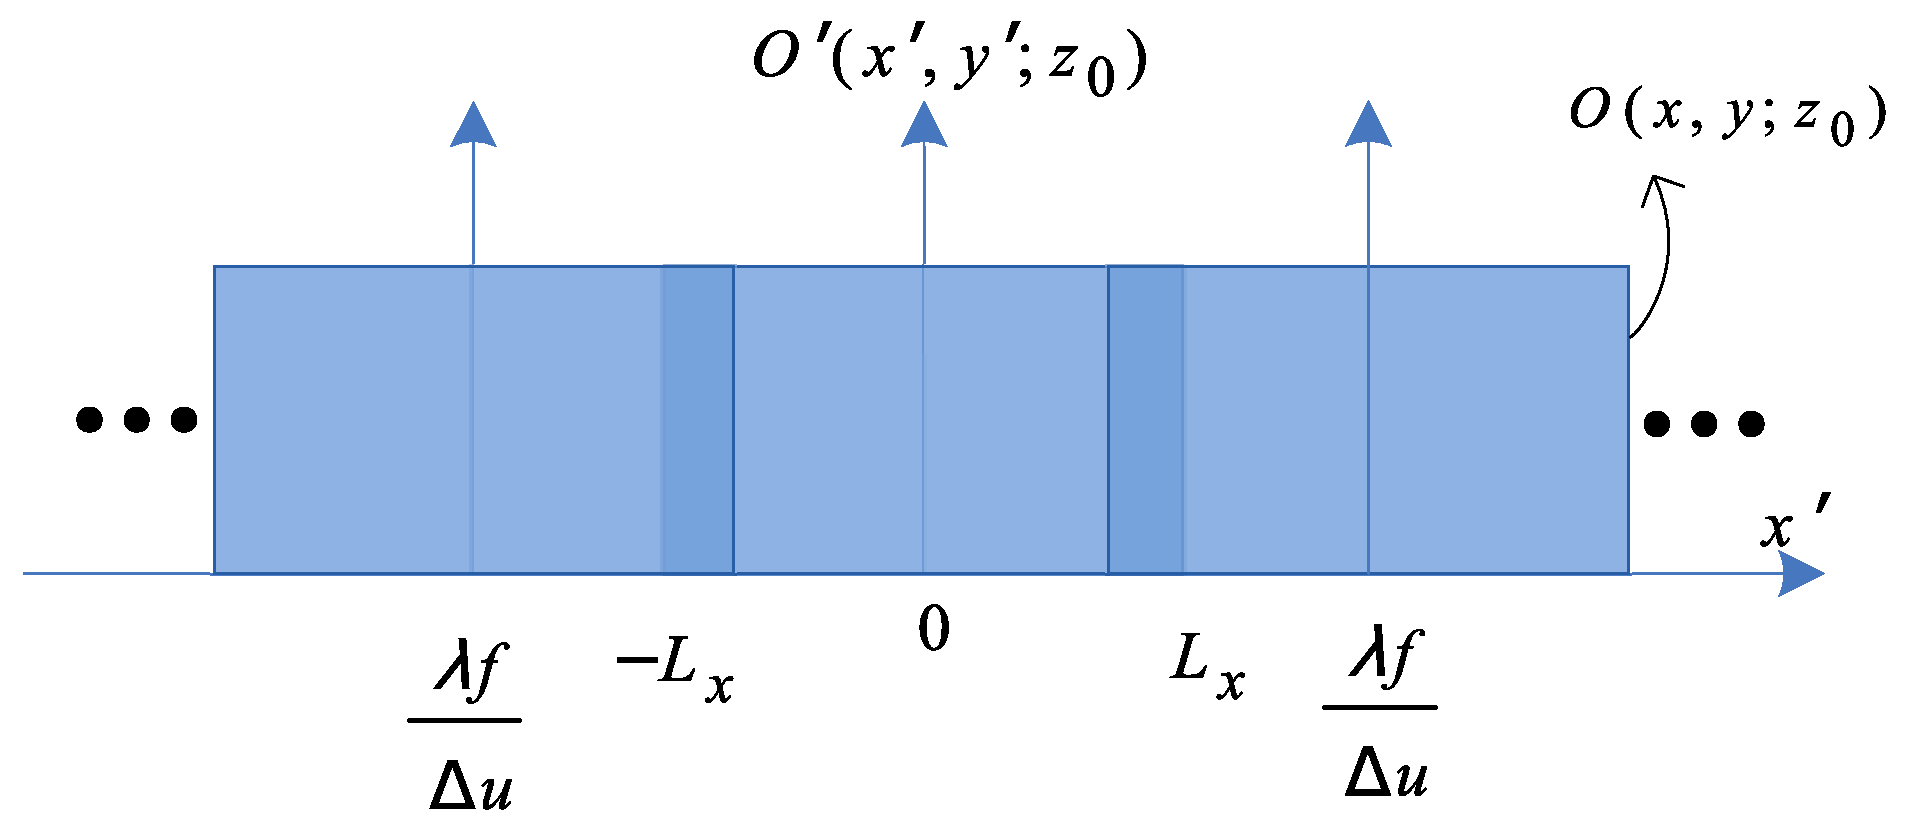
\includegraphics[width=.6\columnwidth]{fig_5}
% \caption{Spatial frequency domain representation of the hologram. (a) Using rectangular lens array. (b)Using hexagonal lens array.}
% \label{fig_5}
% \end{figure}

\begin{figure}[htb]
\centering
	\captionsetup[subfigure]{justification=centering}
	\begin{subfigure}[b]{0.4\linewidth}
	\centering
	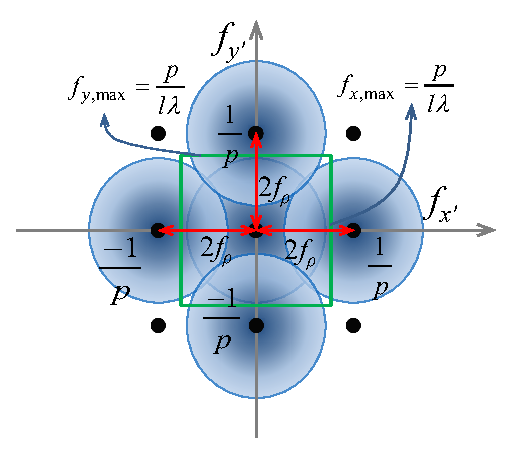
\includegraphics[width=1\columnwidth]{hex_ana_0}
	\caption{}
	\end{subfigure}
	\begin{subfigure}[b]{0.4\linewidth}
	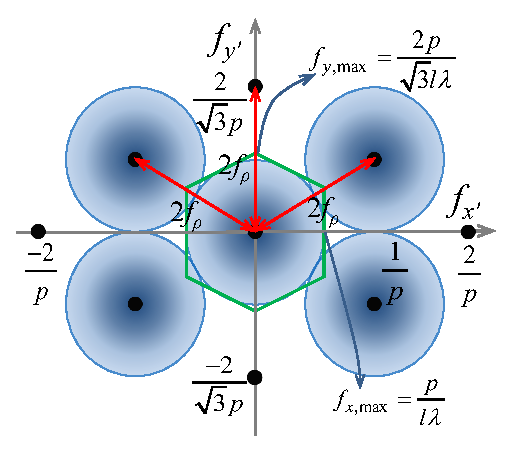
\includegraphics[width=1\columnwidth]{hex_ana_1}
	\centering
	\caption{}
	\end{subfigure}
\caption{Spatial frequency domain representation of the hologram. (a) Using rectangular lens array. (b)Using hexagonal lens array.}
\label{fig_5}
\end{figure}



\subsection{Orthographic image generation using hexagonal lens array}

In the case of using hexagonal lens array, because one orthographic image is the collection of the pixels in each elemental image with the same local position~\cite{Park_2009_OE,Zhang_2006_CSVT,Park_2008_OE}, the pixel distribution of one orthographic image can be represented by Fig.~\ref{fig_6}(a), in which the hexagons mean the elemental image areas. The sampling points of the object, which correspond to the pixel distribution of the orthographic images, are aligned as the filled circles in Fig.~\ref{fig_6}(b). The sampling intervals of the object are $p/2$ along horizontal direction and $\sqrt{3}/2p$ along vertical direction. Here the sampling intervals mean horizontal or vertical distance between neighboring horizontal or vertical lines connecting filled circles. In our implementation, one zero value point is padded as represented by open circles in Fig.~\ref{fig_6}(b) between two filled circles along the horizontal direction. The Fourier hologram is then generated from the orthographic images using the method in ref.~\cite{Park_2009_OE}.
\begin{figure}[htb]
% \centering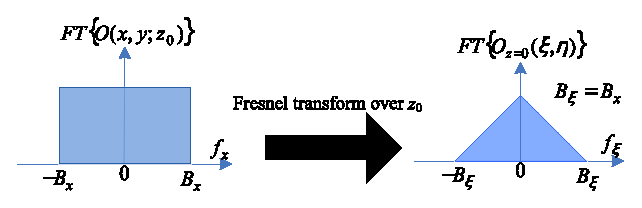
\includegraphics[width=.5\columnwidth]{fig_6}
            \centering
	\captionsetup[subfigure]{justification=centering}
	\begin{subfigure}[b]{0.3\linewidth}
	\centering
	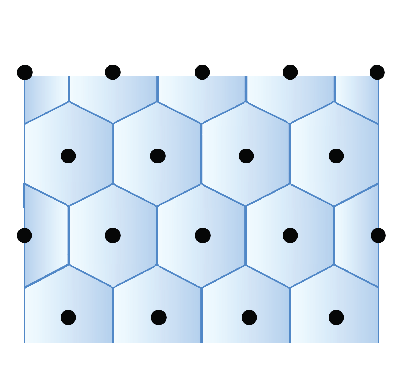
\includegraphics[width=1\columnwidth]{fig6_a}
	\caption{}
	\end{subfigure}
	\begin{subfigure}[b]{0.3\linewidth}
	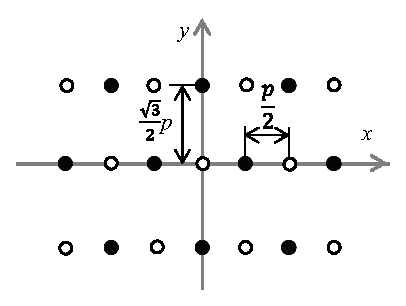
\includegraphics[width=1\columnwidth]{fig6_b}
	\centering
	\caption{}
	\end{subfigure}
\caption{Zero padding method. (a) Pixel distribution in an orthographic image. (b) Zero padding of an orthographic image.}
\label{fig_6}
\end{figure}

In the Fourier hologram generation based on integral imaging, we define the lens pitch of the lens array as the distance between the centers of two adjacent lenses, as Fig. 3 shows. Suppose a rectangular lens array and a hexagonal lens array have the same lens pitch p . Using these two lens arrays, integral Fourier holograms are generated with the method described in Section 2.1. Note that in the integral Fourier hologram method the orthographic image is generated by extracting single pixel per each elemental image. Hence the object field is first sampled with the lens array in the orthographic image generation step and this affects the final hologram resolution. 

\section{Simulation}
Two simulations were performed: one is using rectangular lens array as a reference, and the other is using hexagonal lens array. In the simulations, one plane image was used as the object, as Fig.~\ref{fig_7} shows. The distance from the plane image to the lens array is 50mm. The lens pitch is 1mm. Figure~\ref{fig_8} shows the elemental images. The size of the elemental images is 4000(H)$\times$5000(V) pixels, and the pixel count of each elemental image is 50(H)$\times$50(V) pixels  for  rectangular lens array and 50(H)$\times$58(V) pixels for the hexagonal lens array.
\begin{figure}[htb]
\centering
\includegraphics[width=.2\columnwidth]{fig_7}
\caption{Plane object used in the simulation.}
\label{fig_7}
\end{figure}
\begin{figure}[htb]
\centering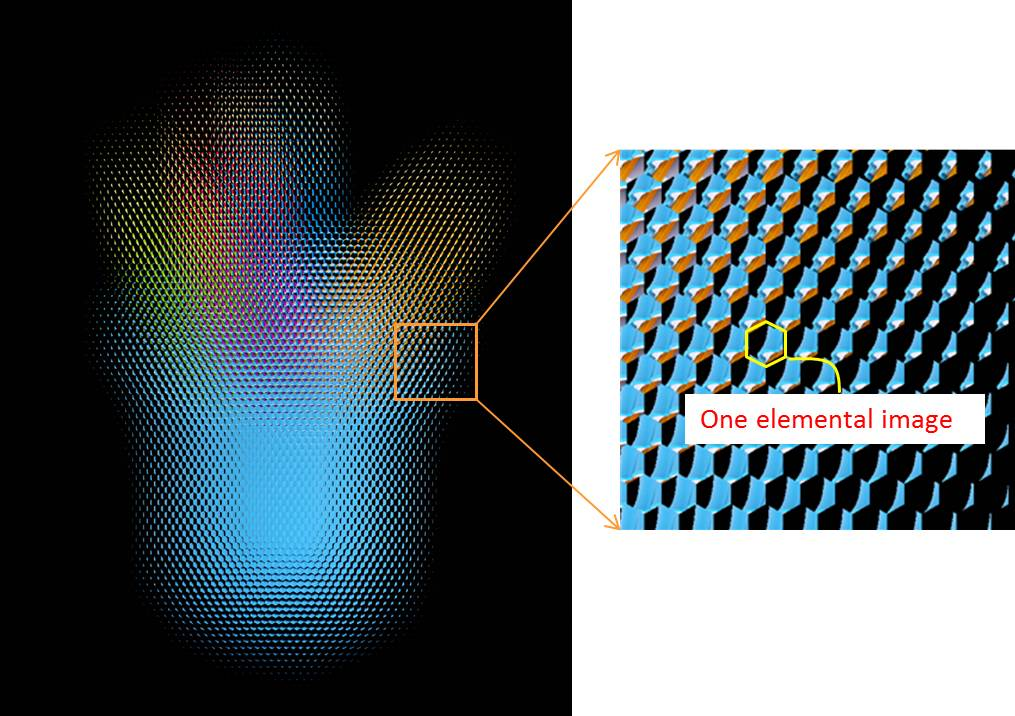
\includegraphics[width=.5\columnwidth]{fig_8}
\caption{Elemental image generated with hexagonal lens array.}
\label{fig_8}
\end{figure}

With the zero padding method described in previous section, orthographic images are generated as Fig. 9 shows. 
\begin{figure}[htb]
\centering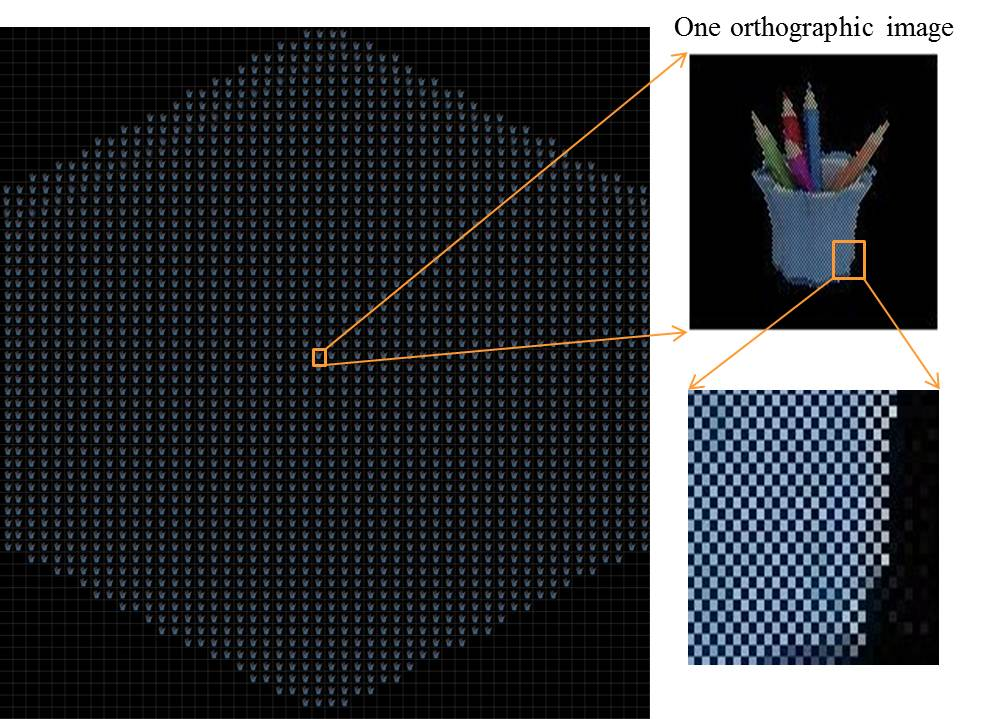
\includegraphics[width=.6\columnwidth]{fig_9}
\caption{Orthographic image generated from the elemental images captured with hexagonal lens array. }
\label{fig_9}
\end{figure}

From the generated orthographic images, holograms of red, green and blue components are generated separately. Figure~\ref{fig_10} shows the amplitude and phase of the holograms generated from the red component. Note that in Fig.~\ref{fig_10}(a) and (c), the contrast was adjusted for better visibility. The red, blue and green images are reconstructed from the three holograms and then synthesized together to get the color reconstruction.

\begin{figure}[htb]
% \centering
\includegraphics[width=.45\columnwidth]{fig_10}
            \centering
	\captionsetup[subfigure]{justification=centering}
	\begin{subfigure}[b]{0.2\linewidth}
	\centering
	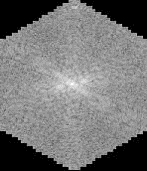
\includegraphics[width=1\columnwidth]{fig10_a}
	\caption{}
	\end{subfigure}
	\begin{subfigure}[b]{0.2\linewidth}
	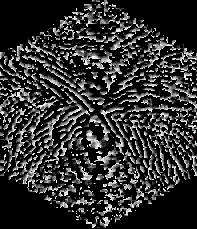
\includegraphics[width=1\columnwidth]{fig10_b}
	\centering
	\caption{}
	\end{subfigure}

	\captionsetup[subfigure]{justification=centering}
	\begin{subfigure}[b]{0.2\linewidth}
	\centering
	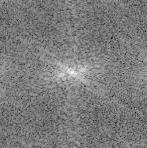
\includegraphics[width=1\columnwidth]{fig10_c}
	\caption{}
	\end{subfigure}
	\begin{subfigure}[b]{0.2\linewidth}
	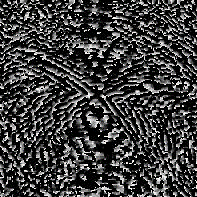
\includegraphics[width=1\columnwidth]{fig10_d}
	\centering
	\caption{}
	\end{subfigure}
\caption{Generated hologram for red component. (a) Amplitude and (b) phase profile of the generated hologram using hexagonal lens array. (c) Amplitude and (d) phase profile of the generated hologram using rectangular lens array.}
\label{fig_10}
\end{figure}
\begin{table}[htbp]
\centering\caption{ Key parameters for the two lens arrays}
\begin{tabular}{p{0.5in}|p{1.2in}|p{0.3in}|p{0.4in}|p{0.45in}|p{0.55in}|p{0.3in}|p{0.3in}} 
% \begin{tabular}{lp{1.7in}|lp{1.7in}} 
\hline 
  & The number of elemental images(V$\times$H) & $\Delta x_p$ & $\Delta y_p$ & $\Delta s=\Delta t$ & $\Delta\theta=\Delta\varphi$ & $\theta_{max}$ & $\varphi_{max}$ \\ \hline 
Rectangle  & $100\times 80$ & 1mm & 1mm & $20\mu m$ & $0.382^\circ$ & $9.55^\circ$ & $9.55^\circ$ \\ \hline 
Hexagon & $116\times 80$ & 1mm & 0.87mm & $20\mu m$ & $0.382^\circ$ & $9.55^\circ$ & $11.03^\circ$ \\ \hline 
\end{tabular}
\label{tb_2}
\end{table}
Table~\ref{tb_2} shows the parameters that are used in the simulations. We compared the reconstructed images of using a hexagonal lens array and a rectangular lens array. Figure 11 shows the magnified results. The images on the right side are the reconstructed images using the hexagonal lens array method and the left images are the reconstructed images using the rectangular lens array method. Aliasing happens in both cases since the elemental lens pitch p is not sufficiently small in comparison with the bandwidth of the object. As expected, due to larger maximum radial spatial frequency and the hexagonal shape of the cut-off spatial frequency region, it can be seen that there are more aliasing in the rectangular lens array case compared to the hexagonal lens array case. In order to measure the resolution improvement, we calculated the peak signal-to-noise ratio (PSNR) and normalized cross correlation~(NCC) between the reconstructed images and the original image. The results are shown in Table~\ref{tb_3}. The resolution improvement is 2.42dB for PSNR and 0.0109 for NCC. 
\begin{table}[htbp]
\centering\caption{PSNR and NCC values of the reconstructed images}
\begin{tabular}{p{0.4in}|p{1.3in}|p{1.2in}|p{0.7in}} \hline 
 & Rectangular lens array & Hexagonal lens array & Improvement \\ \hline 
PSNR & 21.83dB & 24.25dB & 2.42dB \\ \hline 
NCC & 0.9649 & 0.9758 & 0.0109 \\ \hline 
\end{tabular}
\label{tb_3}
\end{table}
\begin{figure}[htb]
\centering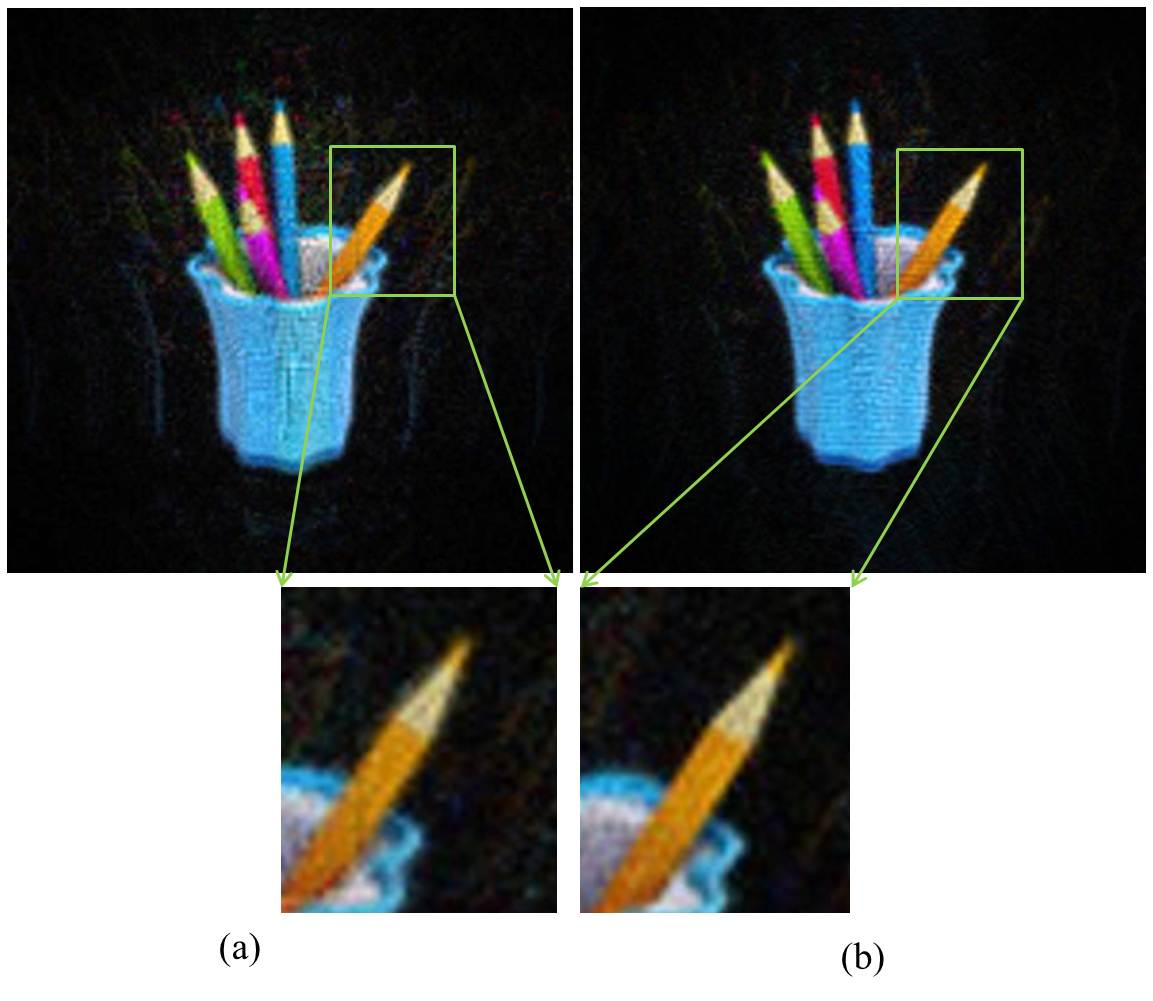
\includegraphics[width=.5\columnwidth]{fig_11}
\caption{Comparison of the reconstructed image. (a) Rectangular lens array case. (b) Hexagonal lens array case.}
\label{fig_11}
\end{figure}

\section{Experiment}
\begin{figure}[htb]
\centering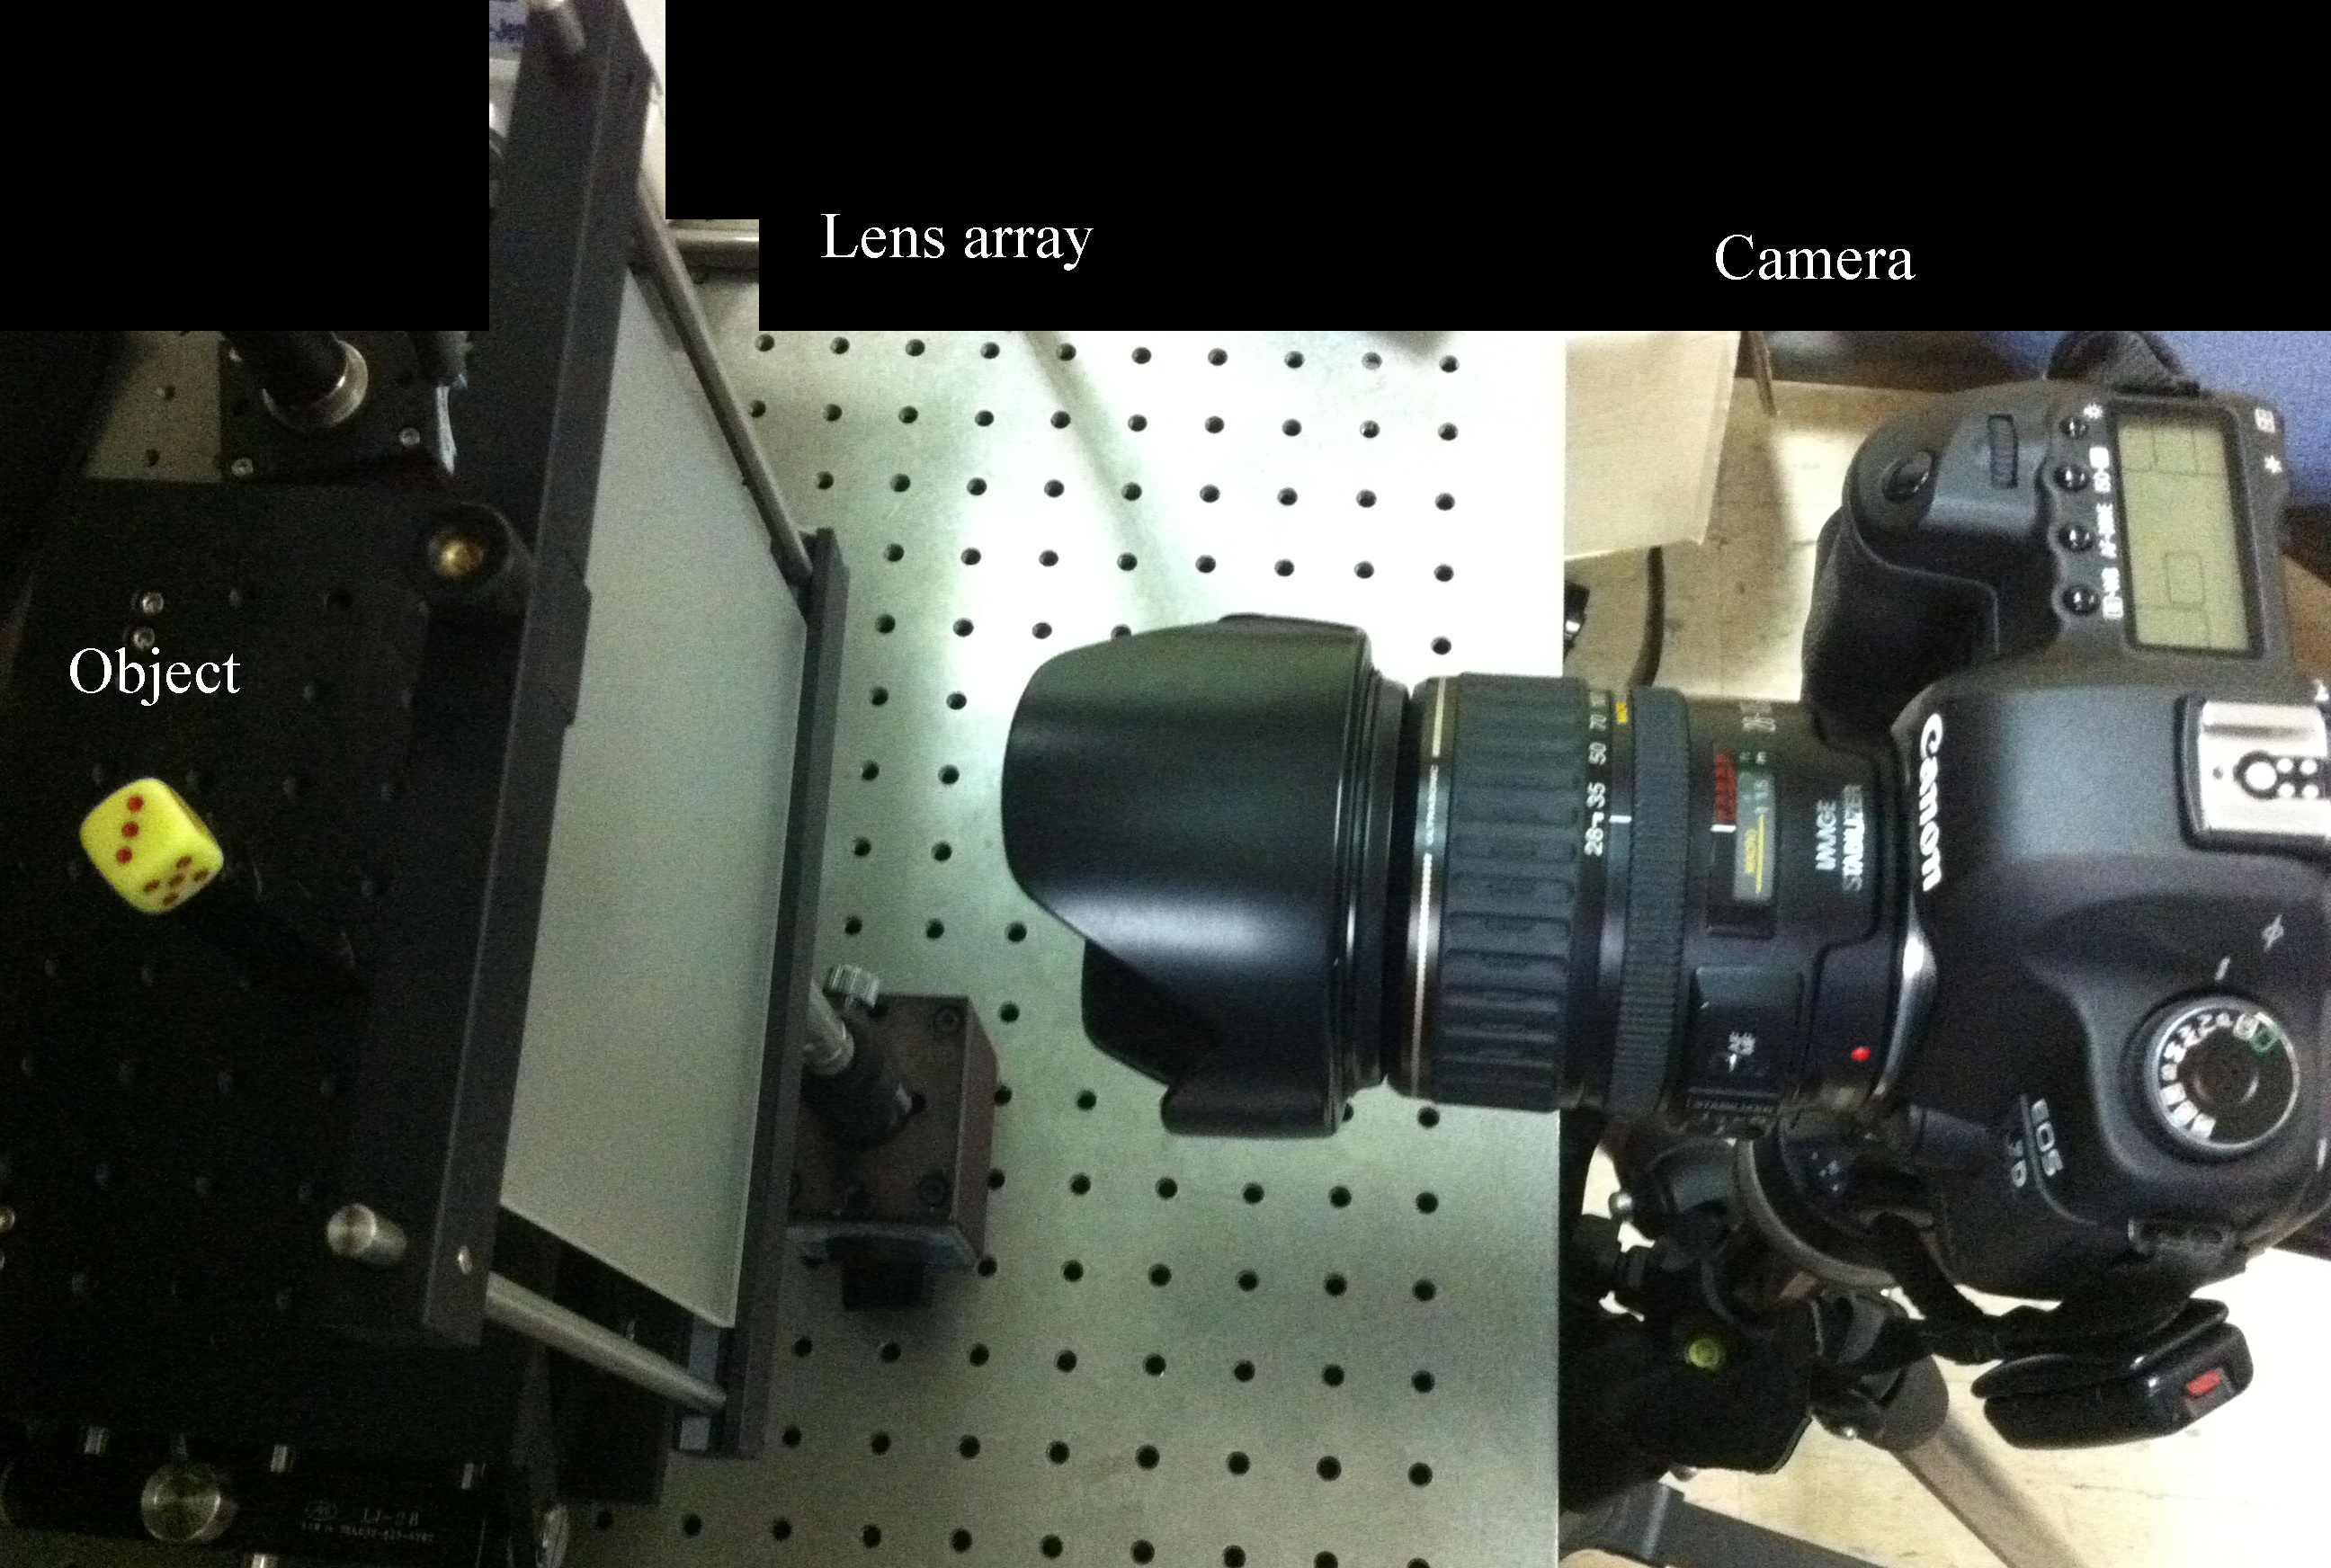
\includegraphics[width=.5\columnwidth]{fig_12}
\caption{Experimental setup for capturing objects.}
\label{fig_12}
\end{figure}
\noindent The theory was also verified experimentally. We performed two experiments, one using rectangular lens array and the other using hexagonal lens array. The setups for capturing the elemental images are the same, as Fig.~\ref{fig_12} shows. The difference is only the lens array shape.  Both the rectangular lens array and the hexagonal lens array have 1 mm lens pitch. The focal length of the two lens arrays is 3.3 mm. The pixel count of the elemental images along the horizontal direction is 58 pixels. 
\begin{figure}[!htb]
% \centering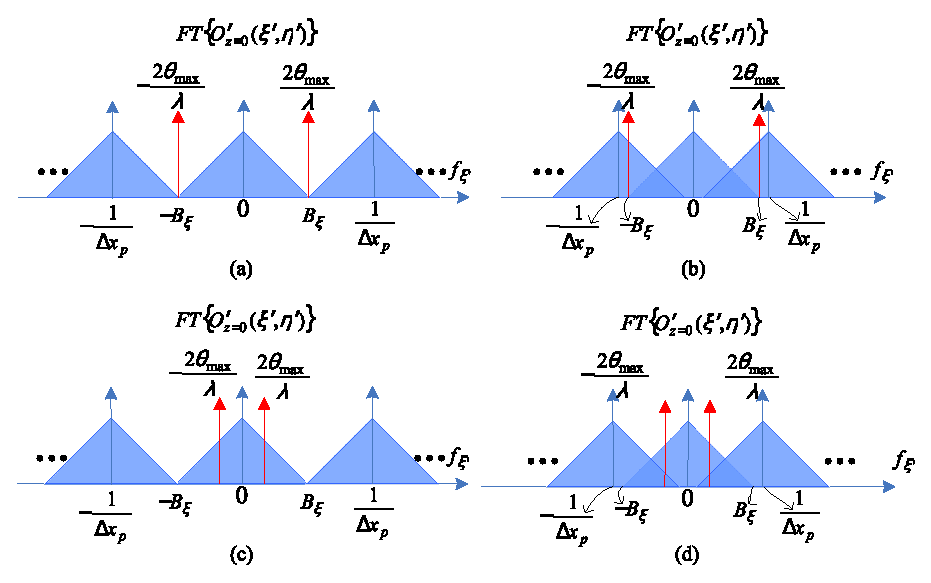
\includegraphics[width=.45\columnwidth]{fig_13}
            \centering
	\captionsetup[subfigure]{justification=centering}
	\begin{subfigure}[b]{0.2\linewidth}
	\centering
	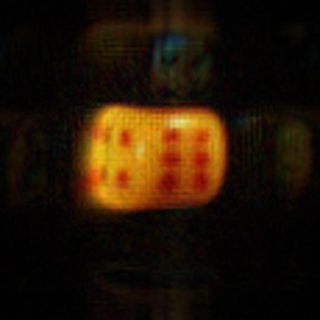
\includegraphics[width=1\columnwidth]{fig13_a}
	\caption{}
	\end{subfigure}
	\begin{subfigure}[b]{0.2\linewidth}
	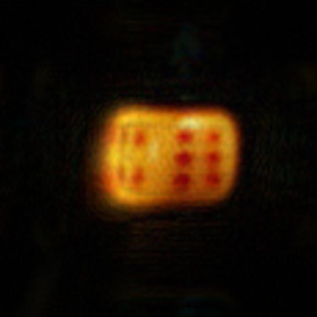
\includegraphics[width=1\columnwidth]{fig13_b}
	\centering
	\caption{}
	\end{subfigure}
\caption{Numerical reconstruction: (a) Rectangular lens array case (Media 1). (b) Hexagonal lens array case (Media 2)}
\label{fig_13}
\end{figure}
  
Figure~\ref{fig_13} shows the movies of the numerical reconstruction at different distances of the generated hologram. It is obvious that the reconstructed images using hexagonal lens array show less aliasing than those using the rectangular lens array.
\begin{figure}[!htb]
% \centering\includegraphics[width=.4\columnwidth]{fig_14}
 \centering
	\captionsetup[subfigure]{justification=centering}
	\begin{subfigure}[b]{0.45\linewidth}
	\centering
	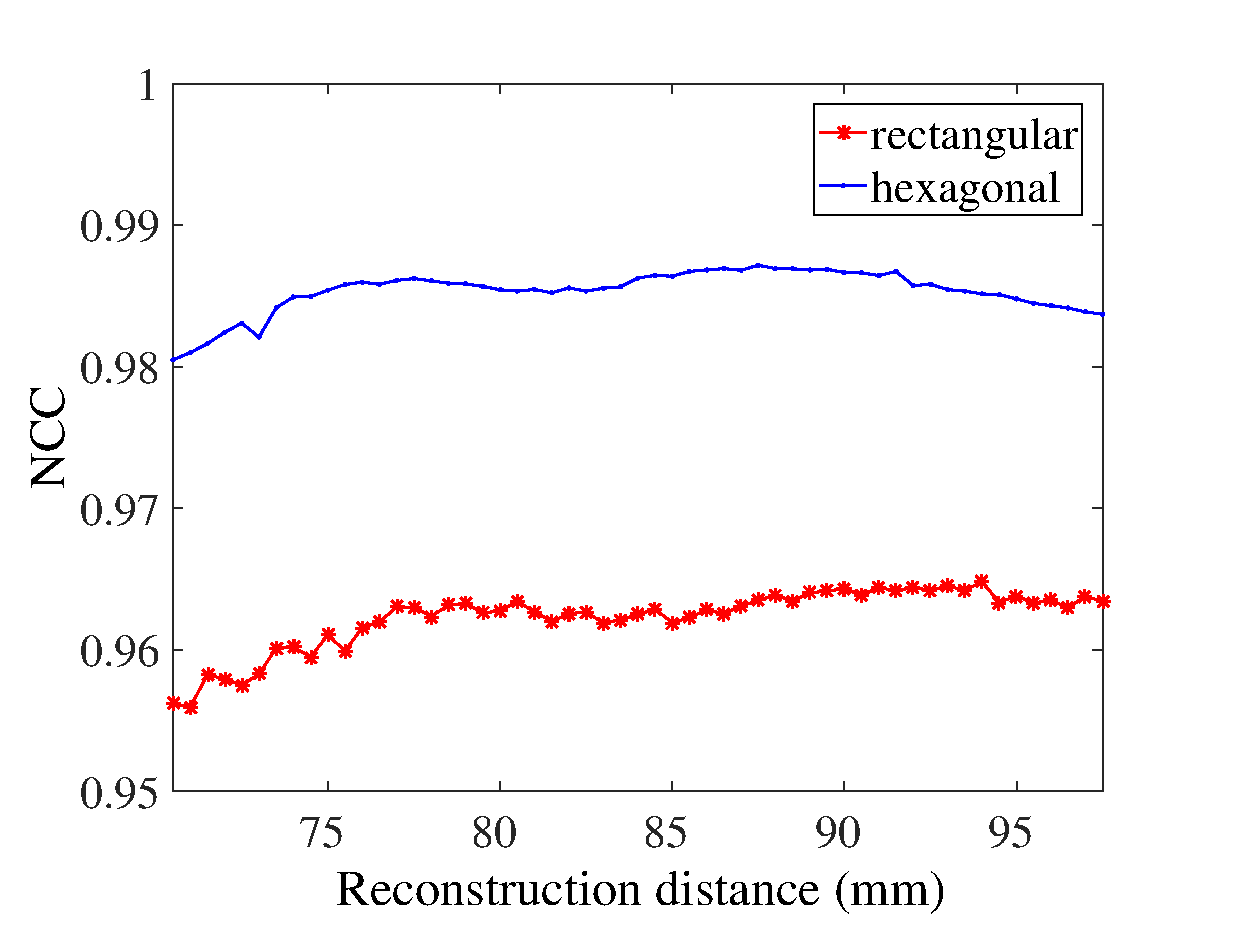
\includegraphics[width=1\columnwidth]{fig14_a}
	\caption{}
	\end{subfigure}
	\begin{subfigure}[b]{0.45\linewidth}
	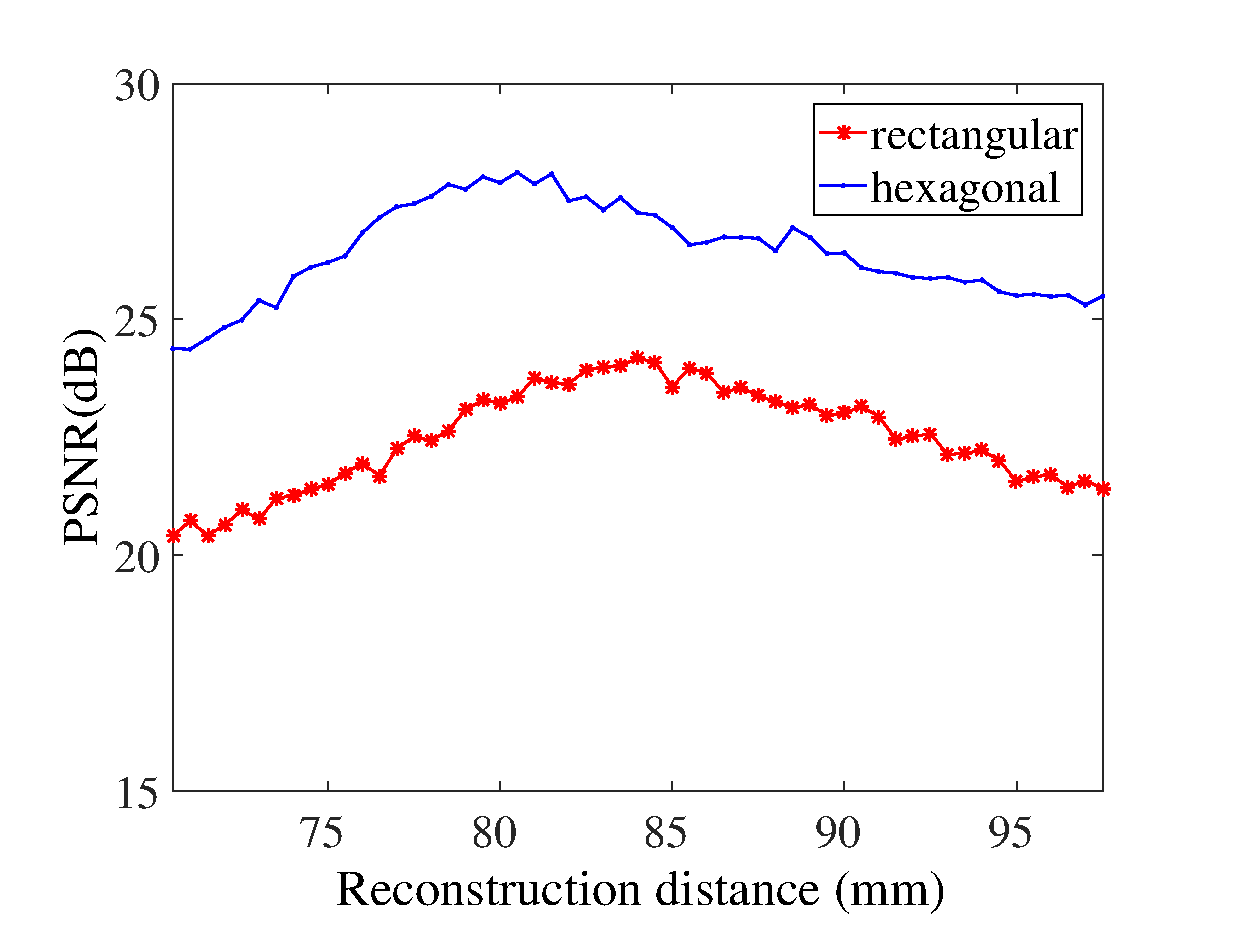
\includegraphics[width=1\columnwidth]{fig14_b}
	\centering
	\caption{}
	\end{subfigure}
\caption{PSNR and NCC of the images reconstructed at different distances. (a) NCC, (b) PSNR. 
}
\label{fig_14}
\end{figure}

To verify the image quality enhancement of the reconstructed images, we calculated the PSNR and NCC values. The results are shown in Fig.~\ref{fig_14}. Figure~\ref{fig_14}(a) shows the PSNR of the reconstructed depth images. The average values are shown in Table 4. The improvement is about 3.94dB. Figure~\ref{fig_14}(b) shows the NCC of the reconstructed depth images. The blue and red lines are the NCC of reconstructed images using hexagonal lens array and rectangular lens array, respectively. The improvement of average NCC is about 0.0230. 
\begin{table}[htbp]
\centering\caption{Average PSNR and NCC values of the reconstructed images}
\begin{tabular}{p{0.4in}|p{1.3in}|p{1.1in}|p{0.7in}} \hline 
 & Rectangular lens array & Hexagonal les array & Improvement \\ \hline 
PSNR & 22.48 dB & 26.42 dB & 3.94 dB \\ \hline 
NCC & 0.9623 & 0.9853 & 0.0230 \\ \hline 
\end{tabular}
\label{tb_4}
\end{table}

\section{Conclusion}
In this paper, we compared the resolution of the hologram reconstruction methods using a rectangular lens array and a hexagonal lens array based on integral imaging. From the sampling theory, it showed that the resolution of the reconstruction is better in the case of using hexagonal lens array than in the case of using rectangular lens array. Both simulation and experiments verified the theoretical expectation.

\section*{Acknowledgments} 
This work was supported by the Brain Korea 21 Program (Information Technology of Seoul National University).

\end{document}
